\documentclass[11pt]{article}

\usepackage[
    left=1.0in,
    right=1.0in,
    top=1.0in,
    bottom=1.0in,
    paperwidth=8.5in,
    paperheight=11in,
]{geometry}

%\usepackage[render]{pdf_poker}
\usepackage{pdf_poker}

\begin{document}

\title{pdf\_poker for \LaTeX{}}

\author{Christopher Donham}

\date{March 26, 2025}

\maketitle

\centerline{
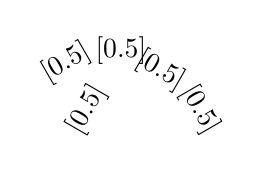
\begin{tikzpicture}
  \node (img1) {\rotatebox{60}{\CardTenClubs[0.5]}};
  \node (img2) at (img1.east) [xshift=-0.7cm, yshift=0.6cm] {\rotatebox{30}{\CardJackDiamonds[0.5]}};
  \node (img3) at (img1.east) [xshift=0cm, yshift=0.75cm] {\CardQueenClubs[0.5]};
  \node (img4) at (img1.east) [xshift=0.5cm, yshift=0.5cm] {\rotatebox{-30}{\CardKingHearts[0.5]}};
  \node (img5) at (img1.east) [xshift=1cm, yshift=0cm] {\rotatebox{-60}{\CardAceSpades[0.5]}};
\end{tikzpicture}}

\section{Introduction}

I am a statistics teacher and use pdflatex with Beamer to create
slides for my lessons.  Playing cards are commonly used to explain
probability, and feature in some of my slides.  A fine library of
playing cards is available in pstricks.  However, Beamer, pdflatex and
pstricks do not interact well.  I also occasionally find other times
when packages I am using in pdflatex do not allow me to use pstricks.
I wrote this package so that I could use playing cards without having
to fight with pstricks.  

\CardAceSpades[0.3]
\CardTwoSpades[0.3]
\CardThreeSpades[0.3]
\CardFourSpades[0.3]
\CardFiveSpades[0.3]
\CardSixSpades[0.3]
\CardSevenSpades[0.3]
\CardEightSpades[0.3]
\CardNineSpades[0.3]
\CardTenSpades[0.3]
\CardJackSpades[0.3]
\CardQueenSpades[0.3]
\CardKingSpades[0.3]

\CardAceHearts[0.3]
\CardTwoHearts[0.3]
\CardThreeHearts[0.3]
\CardFourHearts[0.3]
\CardFiveHearts[0.3]
\CardSixHearts[0.3]
\CardSevenHearts[0.3]
\CardEightHearts[0.3]
\CardNineHearts[0.3]
\CardTenHearts[0.3]
\CardJackHearts[0.3]
\CardQueenHearts[0.3]
\CardKingHearts[0.3]

\CardAceDiamonds[0.3]
\CardTwoDiamonds[0.3]
\CardThreeDiamonds[0.3]
\CardFourDiamonds[0.3]
\CardFiveDiamonds[0.3]
\CardSixDiamonds[0.3]
\CardSevenDiamonds[0.3]
\CardEightDiamonds[0.3]
\CardNineDiamonds[0.3]
\CardTenDiamonds[0.3]
\CardJackDiamonds[0.3]
\CardQueenDiamonds[0.3]
\CardKingDiamonds[0.3]

\CardAceClubs[0.3]
\CardTwoClubs[0.3]
\CardThreeClubs[0.3]
\CardFourClubs[0.3]
\CardFiveClubs[0.3]
\CardSixClubs[0.3]
\CardSevenClubs[0.3]
\CardEightClubs[0.3]
\CardNineClubs[0.3]
\CardTenClubs[0.3]
\CardJackClubs[0.3]
\CardQueenClubs[0.3]
\CardKingClubs[0.3]

\end{document}
